\documentclass[UTF8]{ctexart} % 文档类型为使用ctex宏集的article类型;
\title{政府补贴与企业创新}
\author{朱录}
\date{\today}
\usepackage{amsmath} % 数学公式宏包;
\usepackage{xfrac} %  输入繁分式宏包;
\usepackage{graphicx} % 插入图片宏包;
\usepackage[paperwidth=210mm,paperheight=290mm,left=20mm,right=20mm,top=25mm, bottom=15mm]{geometry} % 页面设置的宏包;
\usepackage[cache=false]{minted}  % 代码高亮;
\usepackage{fancyhdr} %页眉页脚宏包,放在导言区;
\usepackage{cite}
\pagestyle{fancy}
\lhead{朱录}
\chead{2020年3月22日}
\rhead{17839456755}
\lfoot{}
\cfoot{-\thepage-}
\rfoot{}
\renewcommand{\headrulewidth}{0.4pt}
\renewcommand{\headwidth}{\textwidth}
\renewcommand{\footrulewidth}{0pt}
\begin{document}
\maketitle
\tableofcontents
\section{引言}
自2012年党的“十八大”提出科技创新到2016年再次强调创新,对于创新的关注度与日俱增,再到2017年,党的“十九大”将创新作为我国社会主义现代化经济体系的战略支撑,据此可以看出创新驱动发展已经成为当前我国经济结构转型、产业迈向全球价值链高端的重要战略手段。创新作为经济发展的生命力,持续推动着社会不断向前进步,而企业作为创新活动的主体,必须源源不断地将资源转移到创新过程中,正值我国经济由高速增长向高质量发展的转型阶段,新的时代环境下实施创新驱动更是大势所趋,在此背景下研究政府补贴对企业的研发激励效应显然具有重要的现实意义。
\section{文献综述与研究假说}
\subsection{政府补贴对企业创新的影响}
首先,从宏观视角来看,政府补贴通过资源配置影响企业的技术创新。根据公共经济学理论,企业技术创新具有正的外部性特征,相对于社会整体对企业技术创新的需求,私人部门的研发投入总是不足的。企业能够利用的资源是一定的,由于企业的目标是在当前资源约束下的利润最大化,技术创新活动投入的资源多了,影响企业生产等其他方面的资源投入就少了,企业的生产可能性边界并未发生平移。从这个角度出发,政府补贴直接补充了企业缺乏的技术创新资源(Tether, 2002)[14],从而增加了企业总投入,使得企业面临的生产可能性边界右移。在其它条件不变的情况下,最终促进企业进行更多研发和创新活动(Romijn和Albaladejo, 2002; Carboni, 2011 ; Kang和Park, 2012)[15-17]。
其次,从微观视角来看,政府补贴通过改变高管激励进而影响企业的技术创新。与激励一般性质的企业活动不同,激励企业创新面临更大挑战。按绩效激励并对失败进行惩罚的传统合约不足以激励企业进行更多的技术创新活动。从公司治理视角,如何激励企业创新?Manso(2011)[18]的研究认为,激励创新工作需要对短期失败的容忍和对长期的成功给予回报,这样的契约组合才是最能够激励企业创新的。
\subsection{外部监督的调节作用}
以分析师和机构投资者为代表的外部监督会影响企业管理人员的决策行为,进而影响企业技术创新。基于“信息中介”假说的观点认为,外部监督将上市公司创新活动更加全面准确地传递给各类投资者,帮助他们更好地理解公司创新的长期投资价值,公司管理者
\section{研究设计}
\subsection{样本选取}
上市公司专利数据是衡量技术创新的关键数据,由于上市公司的专利数据不需要强制披露,无法从公司财务报表中直接获取,所以需要通过专业数据库来收集。本文的专利数据从大为(INNOJOY)专利数据库获取。大为专利数据库提供了上市公司每项发明专利详实的数据,包括申请年份、授权年份、引证文献和被引证文献等。
\subsubsection{衡量创新}
企业技术创新由创新投入和创新产出两个维度构成。对于创新投入变量,本文参照先前的文献,使用企业研发投入来衡量中国企业技术创新投入。同时为了消除企业规模的影响,更加准确衡量企业创新投入的强度,对企投入事先进行处理,使用企业当入与上一年总资产的比值来衡量企业技术创新投入。
\paragraph{企业技术创新}
企业技术创新由创新投入和创新产出两个维度构成。对于创新投入变量,本文参照先前的文献,使用企业研发投入来衡量中国企业技术创新投入。同时为了消除企业规模的影响,更加准确衡量企业创新投入的强度,对企投入事先进行处理,使用企.
\subparagraph{企业技术创新}
由创新投入和创新产出两个维度构成。对于创新投入变量,本文参照先前的文献,使用企业研发投入来衡量中国企业技术创新投入。同时为了消除企业规模的影响,更加准确衡量企业创新投入的强度,对企投入事先进行处理,使用企
\subsubsection{衡量补贴}
中国政府对企业创新进行补贴的种类很多,例如税收优惠、财政补贴和专项资金等,统计口径也不一致,缺乏统一的披露形式。本文的政府补贴数据除了采用上市公司财务报表中附注“营业外收入”科目下的“政府补贴明细”数据外,还结合网络爬虫和文本分析法,进一步挖掘上市公司公告中的数据,最终汇总得到政府补贴数示。
\subsection{描述统计}
企业技术创新由创新投入和创新产出两个维度构成。对于创新投入变量,本文参照先前的文献,使用企业研发投入来衡量中国企业技术创新投入。同时为了消除企业规模的影响,更加准确衡量企业创新投入的强度,对企投入事先进行处理,使用企
\subsection{实证研究}
企业技术创新由创新投入和创新产出两个维度构成。对于创新投入变量,本文参照先前的文献,使用企业研发投入来衡量中国企业技术创新投入。同时为了消除企业规模的影响,更加准确衡量企业创新投入的强度,对企投入事先进行处理,使用企
\subsection{稳健性检验}
\subsubsection{工具变量}
企业技术创新由创新投入和创新产出两个维度构成。对于创新投入变量,本文参照先前的文献,使用企业研发投入来衡量中国企业技术创新投入。同时为了消除企业规模的影响,更加准确衡量企业创新投入的强度,对企投入事先进行处理,使用企
\subsubsection{匹配}
企业技术创新由创新投入和创新产出两个维度构成。对于创新投入变量,本文参照先前的文献,使用企业研发投入来衡量中国企业技术创新投入。同时为了消除企业规模的影响,更加准确衡量企业创新投入的强度,对企投入事先进行处理,使用企
\section{研究结论}
企业技术创新\cite{林炜企业创新激励}由创新投入和创新产出两个维度构成。对于创新投入变量,本文参照先前的文献,使用企业研发投入来衡量中国企业技\cite{田轩股权激励计划能促进企业创新吗}术创新投入。同时为了消除企业规模的影响,更加准确衡量企业创新投入的强度,对企投入事先进行处理,使用企

\bibliographystyle{plain} % 参考文献样式;
\bibliography{paper_ref.bib} % bib格式的参考文献题录;



$\sqrt{x}$, \quad $\frac{1}{2}$. %插入行内公式

\[ \sqrt{x}, \] % 插入行间公式,不需要编号,如果需要编号可以使用equation环境;
\begin{equation} % 代编号,也可以使用equation*来取消编号;
e = mc^2
\end{equation}

\[ \frac{1}{2}. \]
\[ \dfrac{1}{2}. \]
\[ \tfrac{1}{2}. \]
\[ \sfrac{1}{2}. \] % 行内公式推荐xfrac宏包提供的\sfrac;
\[ \cfrac{\cfrac{1}{1+x}}{\cfrac{2}{1+x^2}}. \]

业技术创新由创新投入和创新产出两个维$ \sum_{i=1}^n i \quad  \prod_{i=1}^n $  % 求和符号和连乘符号,行内公式显示时压缩上下标显示;
业技术创新由创新投入和创新产出两个维$ \sum\limits _{i=1}^n i\quad \prod\limits _{i=1}^n $  %  limits表示不压缩上下标;
\[ \lim_{x\to0}x^2 \quad \int_a^b x^2 dx \] % 行间公式默认不压缩上下标;
\[ \lim\nolimits _{x\to0}x^2 \quad \int\nolimits_a^b x^2 dx \] % nolimits表示行间公式压缩上下标显示;
\[ \iint\quad \iiint\quad \iiiint\quad \idotsint \] % 多重积分的表示方法
\[ (a+b) \]
\[ [(a+b)*c] \]
\[ \{(a+b)*c\} \] % 小括号和中括号可以直接使用,但是大括号需要\进行转义;
\[ \langle x \rangle \] % 尖括号;
\[ \lvert x \rvert \]  % 单竖线;
\[ \lVert x \rVert \] % 双竖线;
\[ \Biggl(\biggl(\Bigl(\bigl((x)\bigr)\Bigr)\biggr)\Biggr) \]
\[ \Biggl[\biggl[\Bigl[\bigl[[x]\bigr]\Bigr]\biggr]\Biggr] \]
\[ \Biggl \{\biggl \{\Bigl\{\bigl\{\{x\}\bigr\}\Bigr\}\biggr\}\Biggr\} \]
\[ \Biggl\langle \biggl\langle \Bigl\langle\bigl\langle\langle x \rangle \bigr\rangle \Bigr\rangle \biggr\rangle \Biggr\rangle \]
\[ \Biggl\lvert \biggl\lvert \Bigl\lvert\bigl\lvert\lvert x \rvert \bigr\rvert \Bigr\rvert \biggr\rvert \Biggr\rvert \]
\[ \Biggl\lVert \biggl\lVert \Bigl\lVert\bigl\lVert\lVert x \rVert \bigr\rVert \Bigr\rVert \biggr\rVert \Biggr\rVert \] % 由小到大分级括号的显示方法;

\[ x_1,x_2,\dots,x_n\] % 带下标时的省略号;
\[1,2,\cdots,n\ \] % 不带下标时的省略号;
\[1,2,\vdots,n\ \] %竖向省略号;
\[1,2,\ddots,n\ \] % 斜向省略号;

\[ \begin{pmatrix} a&b\\c&d \end{pmatrix} \] % 小括号表示的矩阵,\\表示换行;
\[ \begin{bmatrix} a&b\\c&d \end{bmatrix} \] % 中括号表示的绝阵;
\[ \begin{Bmatrix} a&b\\c&d \end{Bmatrix} \] % 大括号表示的绝阵;
\[ \begin{vmatrix} a&b\\c&d \end{vmatrix} \] % 单竖线表示的绝阵;
\[ \begin{Vmatrix} a&b\\c&d \end{Vmatrix} \] % 双竖线表示的绝阵;
$( \begin{smallmatrix} a&b\\c&d \end{smallmatrix} )$ % 行内小括号表示的绝阵;

\begin{multline} % 不需要对齐的长公式,但是有编号;
  x = a+b+c+{} \\
  d+e+f+g
  \end{multline}

\begin{gather} % 无需对齐的公式组,有编号;
2x+3y = 10 \\
3x+4y = 14
\end{gather}

\[\begin{aligned} %对齐的公式组,需要包含在数学环境之内,有编号,如果不需要编号,使用*号;
a &= b+c+d \\
a+d &= e+f
\end{aligned} \]

\[ y = \begin{cases} %分段函数,以,号对齐;
-x+1&,\quad x\leq 0 \\
x^2+3&,\quad x>0
\end{cases} \]

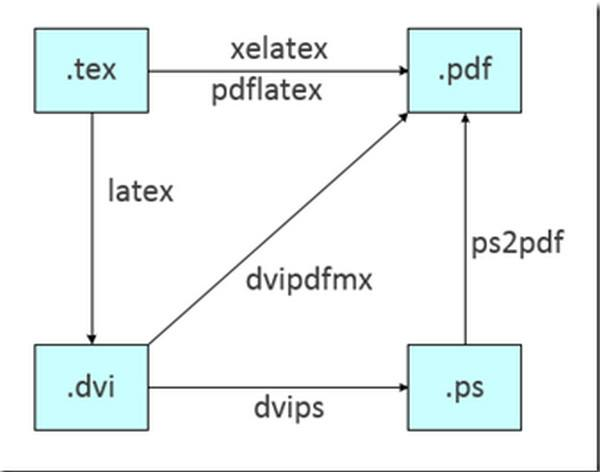
\includegraphics[width = .9\textwidth]{a.jpg} %借用graphicx宏包,插入图片,同源目录下有a.jpg图片就行,不仅仅支持.eps格式的图片;

\begin{tabular}{|l|c|r|} % 三列表格,分别左中右对齐;
\hline % 横线
操作系统 & 发行版 & 编辑器 \\
\hline
windows & MikTeX & TeXMakerx \\
\hline
unix/linux &TeTeX & Kile \\
\hline
Mac OS & MacTeX & TeXShop \\
\hline
通用 & TeX Live & TeXworks \\
\hline
\end{tabular}

\begin{figure}[htbp] % 浮动体,表格和图需要不断调整它们的位置;
\centering % 居中
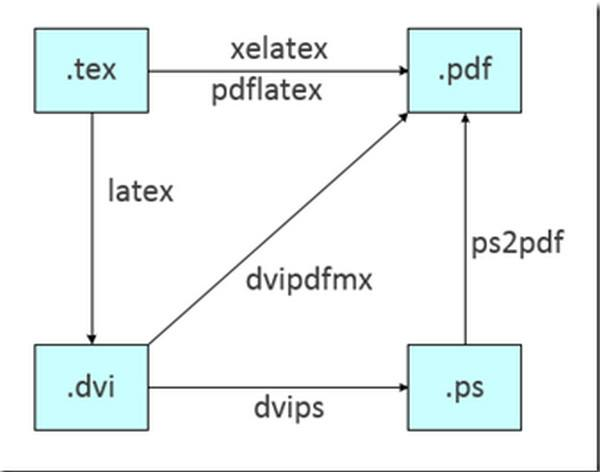
\includegraphics[width = .8\textwidth]{a.jpg} % 80%页面宽度显示图片
\caption{有图有真相} % 图标题
\label{fig:myphoto}
\end{figure}

%\newgeometry{papersize={20cm,15cm}}  %geometry宏包提供的修改页面的命令;
%\newgeometry{left =1cm,right =2cm,top =3cm,bottom =4cm}
%minted代码块语法高亮宏包,需要使用--shell-escape参数;
\begin{minted}{c++}
int main() {
    printf("hello, world");
    return 0;
}
\end{minted}

\begin{minted}[mathescape,
               linenos,
               numbersep=5pt,
               gobble=2,
               frame=lines,
               framesep=2mm]{csharp}
  string title = "This is a Unicode π in the sky"
  /*
  Defined as $\pi=\lim_{n\to\infty}\frac{P_n}{d}$ where $P$ is the perimeter
  of an $n$-sided regular polygon circumscribing a
  circle of diameter $d$.
  */
  const double pi = 3.1415926535
\end{minted}


\end{document}
